\section{ Models setup}

In this section, we explain the details of models which are used in this study.  These models include physics-based ground motion simulation domains, seismic sources, \qsvs{} relationships, ANNs as surrogates, and GA optimization process.  

\subsection{Idealized Domains}

To test the proposed method, we use four different idealized domains. Idealized domains are essential because we have a control on shear wave velocity of the domains. This study's idealized domains are homogeneous and layered. Fig.~\ref{fig:3d_domain_scenarios} represents these domains and seismic velocity,density and depth of layers.  The simulation domain is a cubical box (32.8*32.8*8.2~km). All idealized domains have the same source and 17 stations locations. However, they have different velocity models. The homogenous half space (H1) is the simplest one. We add a shallow (256~m) low velocity layer to H1 domain. This Layer adds some complexity to the homogenous domain. We call this domain L1. In order to study the effect of layer thickness in the results, we modify L1 into L2 domain by increasing the depth of low velocity zone from 256 to 1024~m. The last layered domain includes three layers with 2000, 1000, and 500~m/s shear wave velocity, respectively.  

 \begin{figure}[ht]
    \centering
    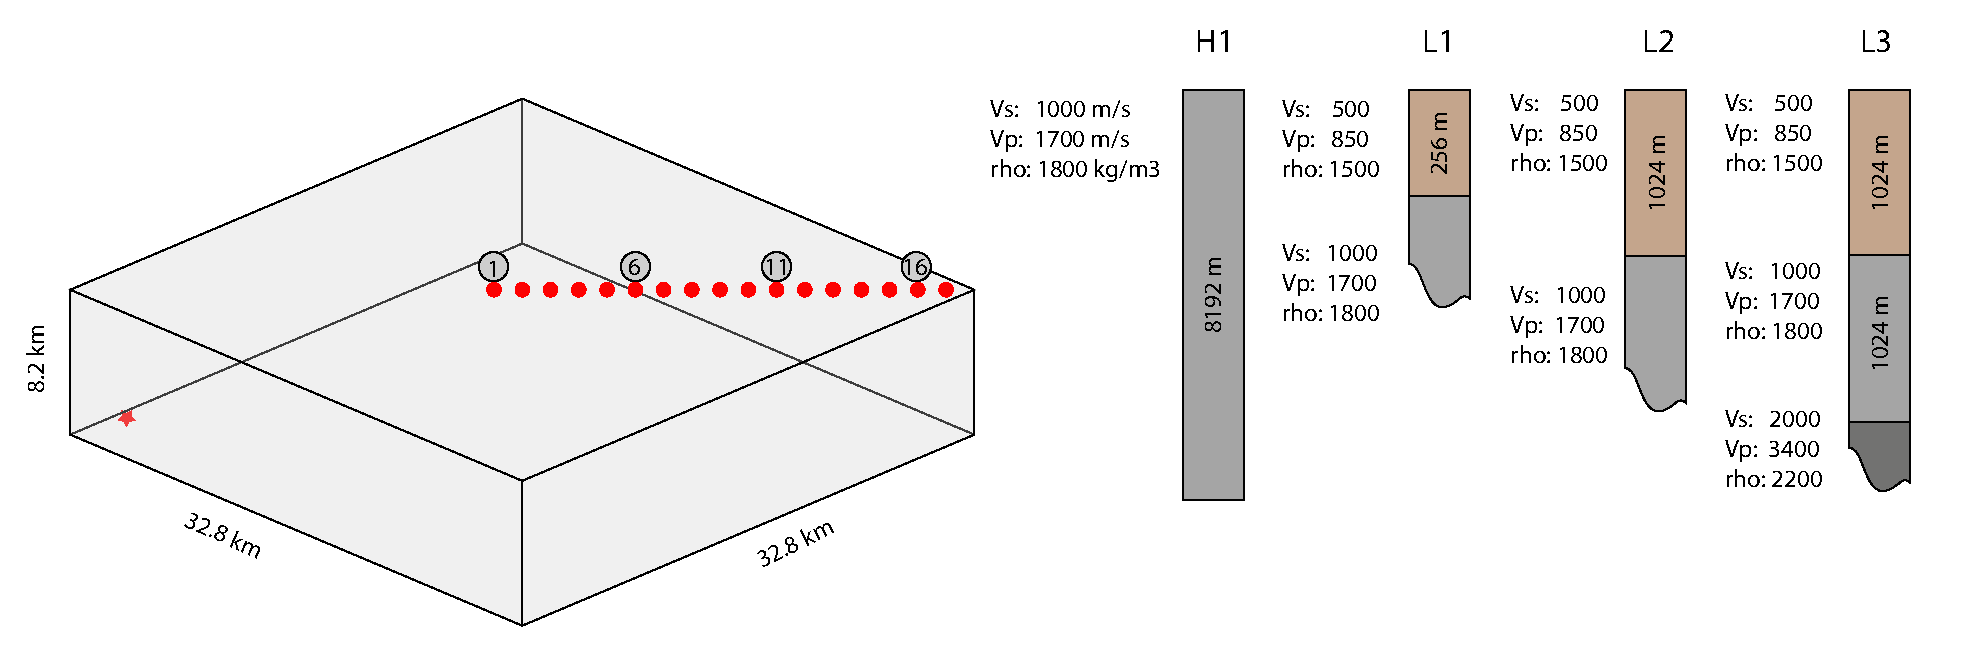
\includegraphics[width=\textwidth]{figures/pdf/Figure_05.pdf}
    \caption{Idealized domains to test the proposed method. Earthquake source is shown with star (2048,2048,7168). Station are at the surface and the numbers are referred in the text. All four idealized case share the same domain dimension with different velocity models.}
    \label{fig:3d_domain_scenarios}
\end{figure}

We run ground motion simulations for each of these domains based on known damping parameters. Using the synthetic generated data as a target values at each station we search for the initially used \qsvs{} relationship parameters to see if the optimization process can find the initially used parameters. The idealized domains are used to confirm the accuracy of the optimization process. We modeled each seismic event with a point source model with seismic moment that is tailored for magnitude $Mw~3.5$. Fig.~\ref{fig:record_section_1000} represents the record section of NS horizontal component for peak ground velocity in H1 domain. The record of each stations are shown according to their hypocenteral distance from the source. Dashed lines show \vp{} and \vs{} arrival times. Peak amplitude of P and S wave of each station can be detected after dashed lines. 

  \begin{figure}[ht]
    \centering
    \includegraphics[width=0.8\textwidth]{figures/pdf/Figure_06.pdf}
    \caption{Record section of NS component of H1 domain. Amplitudes are scaled for better representations.}
    \label{fig:record_section_1000}
\end{figure}

Fig.\ref{fig:record_section_2000_1000_500} represents the record section of NS horizontal component for peak ground velocity in L3 domain. Dashed lines show \vs{} for 2000 and 1000~m/s. 

  \begin{figure}[ht]
    \centering
    \includegraphics[width=0.8\textwidth]{figures/pdf/Figure_07.pdf}
    \caption{Record section of NS component of L3 domain. Amplitudes are scaled for better representations.}
    \label{fig:record_section_2000_1000_500}
\end{figure}

Reflected waves from different layer makes it difficult to choose the peak ground velocity for S wave arrival. The complexity of the other two idealized domains lay between the shown results. 

\subsection{Heterogenous Domain}

Heterogenous domain has a significant difference from idealized ones. In heterogeneous domains, we do not know the effective shear wave velocity of each station. Each station can have some range of effective shear wave velocity. In a heterogeneous domain, depending on effective shear velocity of each station, waves arrive in different times. The heterogeneous region used in this study has greater Los angeles area and also it includes many small basins in different parts. Numerous earthquake recorded in this area and different ground motion simulation studies are conducted for the region for different events; and several velocity models are developed \citep[e.g., see][]{Taborda_2013_BSSA,Taborda_2014_BSSA,Small_2017_SRL}. Fig.~\ref{fig:Figure_stations} shows the  heterogeneous domain and stations location. 

 \begin{figure}[ht]
    \centering
    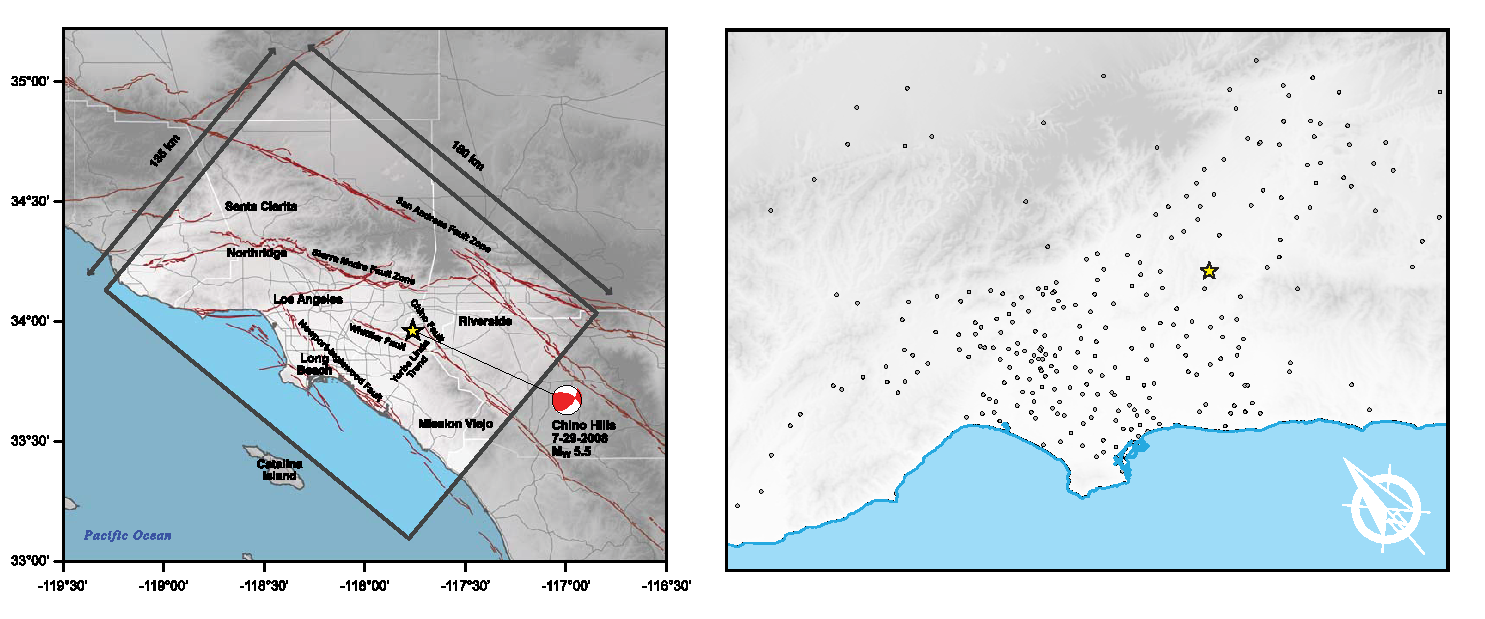
\includegraphics[width=\textwidth]{figures/pdf/Figure_08.pdf}
    \caption{Left: Region of interest and epicentral location of the 2008 Chino Hills earthquake. Major quaternary faults in the area are shown in the back along with the main roads and county divisions. Right: Simulation are of interest. Dots indicate the location of the 262 stations considered in this study for optimization process. {\color{red} Stations that are used in the study will be marked on this figure.}}
    \label{fig:Figure_stations}
\end{figure}

In order to test the methodology with real observational data, we use 2008 $Mw~5.4$  ChinoHills earthquake as an observation platform. Chino Hills earthquake is recorded at more than 300 stations. however we only use the Center for Engineering Strong Motion Data, where there are 262 stations within this study simulation box. We modeled the seismic event with a point source model according to \citep{Taborda_2016_GJI}. Table~\ref{tab:event_details}  and Table~\ref{tab:sim_param} represent the event and simulation details, respectively. 


\begin{table}[ht]
\centering
\caption{Event details}
\label{tab:event_details}
\renewcommand{\arraystretch}{0.75}
\begin{tabular}{lr}
\\ \hline
Name                                 &   Chino Hills                          \\
Origin Time                        & 29 July 2008 , 11:42 AM             \\
Magnitude                          &  Mw 5.4            \\
Moment                             & 1.566751e+17 Nm             \\
Location/Depth                  &  -117.7613 33.9530 14.7 $Km$    \\
Strike/Dip/Rake                 & 47/51/32                                   \\
3D Crustal Model              & SCEC CVM-S4.26                   \\
Source Model                   & Point Source                                  \\ \hline
\end{tabular}
\end{table}


\begin{table}[ht]
\centering
\caption{Simulation Parameters}
\label{tab:sim_param}
\renewcommand{\arraystretch}{0.75}
\begin{tabular}{lr}
\\ \hline
Domain                              &                              \\
~~Length/Width/Depth       & 180,135,61.875 km \\
~~Southwest corner          & -119.288842, 34.120549             \\
~~Northwest corner           & -118.354016, 35.061096             \\
~~Northeast corner            & -116.846030, 34.025873              \\
~~Southeast corner           & -117.780976, 33.096503               \\
~~Rotation Angle               & 39.9 \\
~~Studied records             & 262 \\
Spatial Resolution              &    \\
~~Maximum frequency     & 1 $Hz$ \\
~~Minimum $V_s$            & 350 m/s \\
~~Points per wavelength   & $9\leq p < 14$\\
~~Minimum size element   & 21.9727 $m$\\
~~Maximum size element   & 351.5625 $m$\\
~~Number of elements       & 157209765 \\
~~Number of nodes            & 180080443 \\
~~Number of dangling nodes & 23681911 \\
Time resolution  & \\
~~Simulation $\Delta$t & 0.002 \\
~~Simulation time & 100 s\\ \hline
\end{tabular}
\end{table}

\subsection{Artificial Neural Networks}

We use 1000 combination of randomly generated $C$, $\alpha$, and $\beta$ to develop training data for ANNs. Each training data is the result of running a physics-based ground motion simulation on the domains. Fig.~\ref{fig:Figure_training_data_statistics} shows statistical distribution of the generated data.

 \begin{figure}[ht]
    \centering
    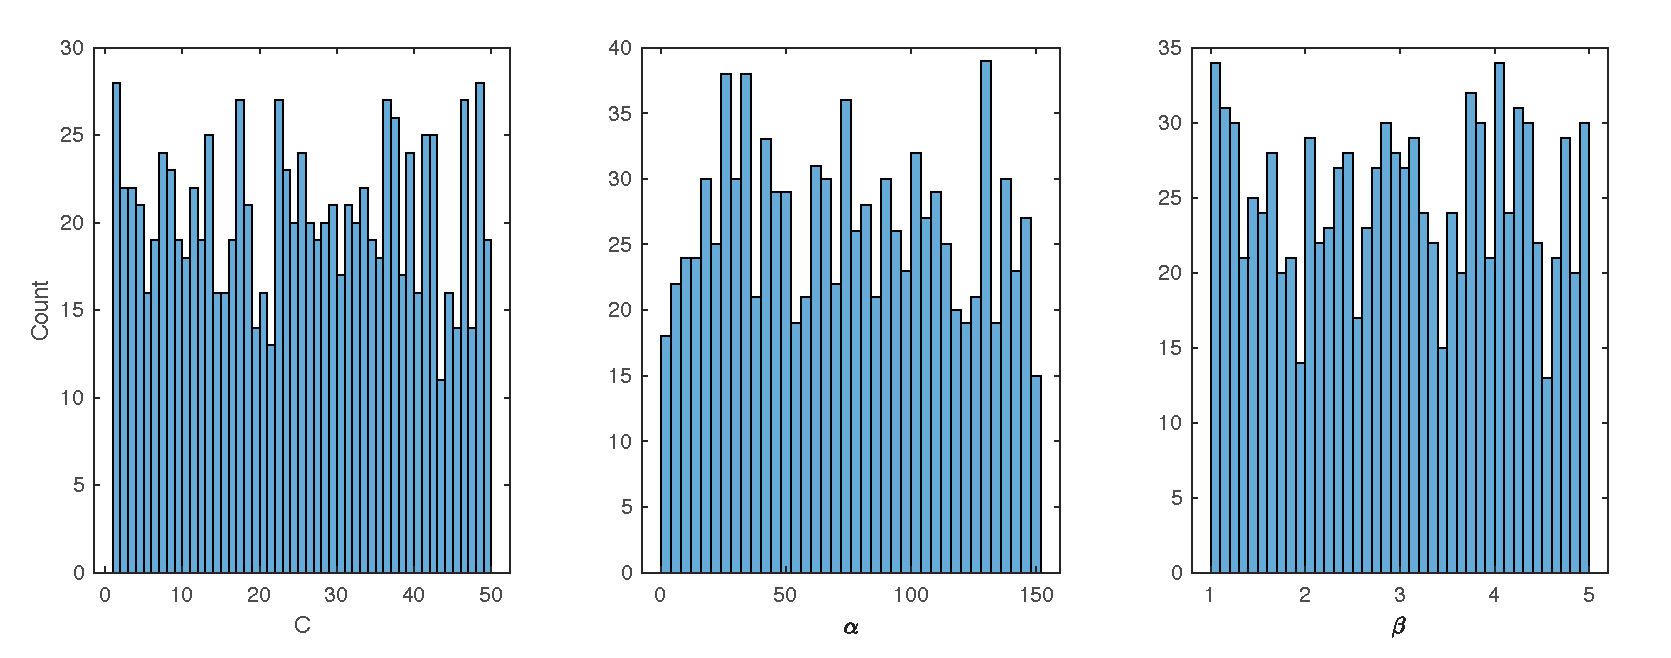
\includegraphics[width=\textwidth]{figures/pdf/Figure_09.pdf}
    \caption{Distribution of \qsvs{} relationship input parameters (i.e. $C$, $\alpha$, and $\beta$) which are used in generating 1000 training data for ANNs.}
    \label{fig:Figure_training_data_statistics}
\end{figure}

 Our analyses show that, defining higher $C$ values (more than 50) compromise the functionality of the network. The reason is, higher $Q$ values provide almost the same signal parameters independent of the input values. Moreover, according to Table~\ref{tab:table_qs} almost all models proposed lower $Q$ values for low velocity zones. Most of previous studies show that $Q$ value increases with increasing shear wave velocity, therefore, we consider $\beta$ to be in the the range of $[1,5]$. Suggested values for $\alpha$, mostly, is between 50--100; we broaden the search domain and use $[0,150]$ as a range of $\alpha$ variation. Therefore, each station of simulation has 1000 training data. Fig.~\ref{fig:Figure_training_data} illustrates that the generated training data can cover almost the whole range of \qsvs{} relationships. Values of Table~\ref{tab:QsVstable} and Fig.~\ref{fig:Figure_q_models} are shown as a thicker black line. The simulation \vsmin{}=350~m/s, therefore, the part of a line which is partially not covered is out of the target velocity zone of this study. 

 \begin{figure}[ht]
    \centering
    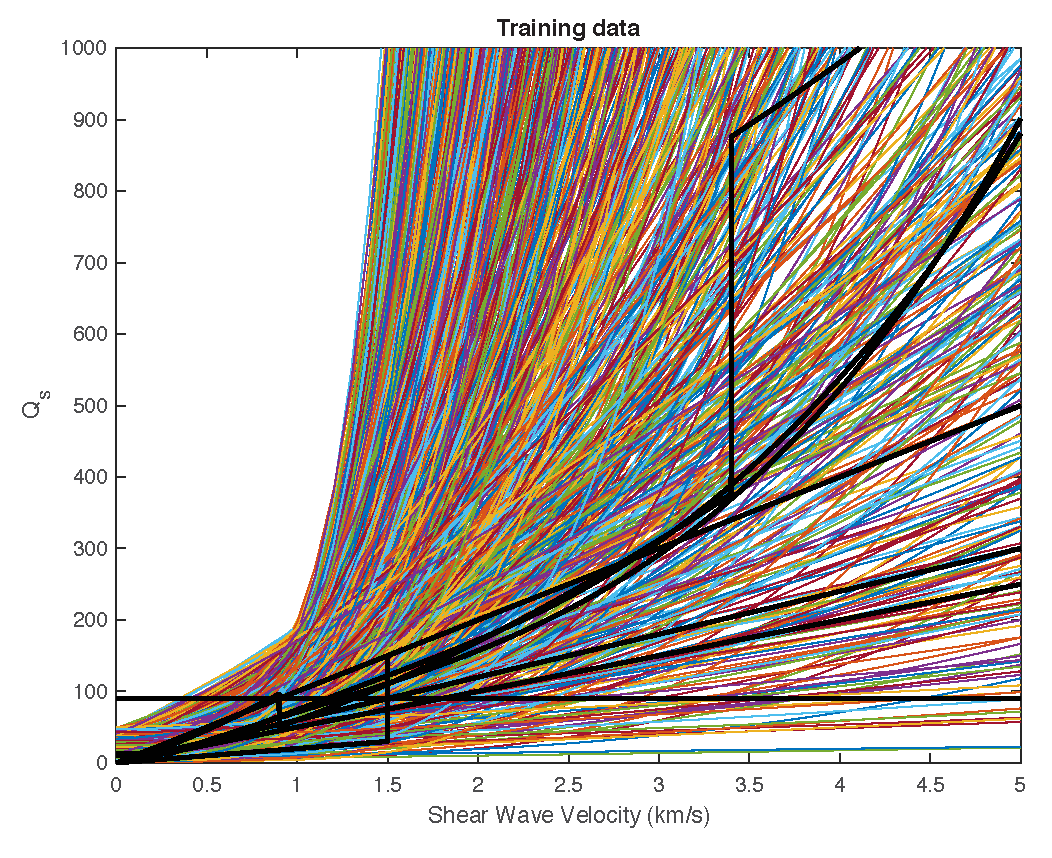
\includegraphics[width=0.5\textwidth]{figures/pdf/Figure_10.pdf}
    \caption{Training data is generated based on 1000 random combination of $C$, $\alpha$, and $\beta$. For statistical distribution of the input parameters refer to Fig.~\ref{fig:Figure_training_data_statistics}. Thick black lines are transferred from Fig.~\ref{fig:Figure_q_models} and represented only for comparison purposes.}
    \label{fig:Figure_training_data}
\end{figure}

 Fig.~\ref{fig:Figure_training_performance} represents the training performance for one of the networks (predicting eight output parameters).


  \begin{figure}[ht]
    \centering
    \includegraphics[width=\textwidth]{figures/pdf/Figure_11.pdf}
    \caption{a) Train, Validation, and Test performance. The circle shows the start of RMSE value for the validation dataset which means overfitting occurs. b) Error histogram}
    \label{fig:Figure_training_performance}
\end{figure}

Fig.~\ref{fig:Figure_training_performance}.a shows the performance of the network for train, validation, and test datasets with respect to epoch.  In the presented training session, after epoch 140, overfitting occurs because training data error decreases, however, validation data error increases. Training session stops based on user defined termination criteria. In this example, since ANN cannot overcome the overfitting problem (validation dataset error still not improving) after 100 more iterations, the learning process stops and the best network that acquired at epoch 140 is returned to the user. Toward bagging approach, we generate 10 different ANNs and use the average value of their predictions. For each ANN, training and validation data are randomly set. Therefore, these networks are trained for different combination of data. Fig.~\ref{fig:Figure_ANN_num_training_data_sens}.a shows that increasing the number of training data, in general, reduce the RMSE for test dataset. Fig.~\ref{fig:Figure_ANN_num_training_data_sens}.b represents accuracy of training network with 100, 400, and 1000 training data on the test dataset. In the figure, the red cross shows results of each individual ANN, the blue circles represent the value of observations and green stars are average of 10 ANNs. In the case with 100 training data, each individual network results (red crosses) is far from the actual value (blue circles), however, bagging approach average them out (green stars) which leads to better fit with actual value. 

  \begin{figure}[ht]
    \centering
    \includegraphics[width=0.8\textwidth]{figures/pdf/Figure_12.pdf}
    \caption{a) Variation of RMSE with increasing number of training data; b)Examples of predicting target value in actual simulation with 100, 400, and 1000 training data. The networks are tested using testing dataset. RMSE scores computed using bagging results.}
    \label{fig:Figure_ANN_num_training_data_sens}
\end{figure}

\subsection{Variation of Alternative Metric Results}
As we mentioned earlier, defining alternative metrics increase signal uniqueness. The variation of input parameters (i.e., $C$,$\alpha$,and $\beta$) are constant for all signal metrics. Since we have all training data and respective ground motion results for each domain, we take a look at variation of alternative metrics for each metric and domain. We use coefficient of variation (CV) as a measure of relative variability of metrics. Since input parameters are the same for all signals and simulation we can safely compare CV for different metrics without further analysis. Coefficient of variation is defined as 

\begin{equation}
CV=\sigma/\mu * 100. 
\end{equation}

High CV indicates that the metric is very sensible to input parameters and provides high variability around the mean value. As a result, high CV means better training of ANN and consequently efficient optimization process. Fig.~\ref{fig:metrics_sensitivity} shows CV for 4 different stations of idealized domains. 

  \begin{figure}[ht]
    \centering
    \includegraphics[width=0.8\textwidth]{figures/pdf/Figure_13.pdf}
    \caption{Coefficient of Variation of different metrics for 1000 training data. Symbols indicates different stations. See Fig.~\ref{fig:3d_domain_scenarios} for stations location.}
    \label{fig:metrics_sensitivity}
\end{figure}


Several points are worth mentioning from Fig.~\ref{fig:metrics_sensitivity}. In all domains, CV increases with increasing distance from source. It suggests the idea that far stations can be trained more accurately and they are much more sensitive to the variation of input parameters. The results prove to be true. As distance of stations increases from source, waves have more time to travel in the medium and this means more time to get affected through domain anelasitisiy. In the simple cases (H1,L1, and L2) response spectra at 1 second (SA1) is more variable, whereas in complicated case (L3) the envelop becomes important. 




%Testing of the proposed method is inspired from checkerboard resolution tests idea from inversion studies \citep[e.g., see][]{liang2008ambient}. 


